


\tikzset{every picture/.style={line width=0.75pt}} %set default line width to 0.75pt        

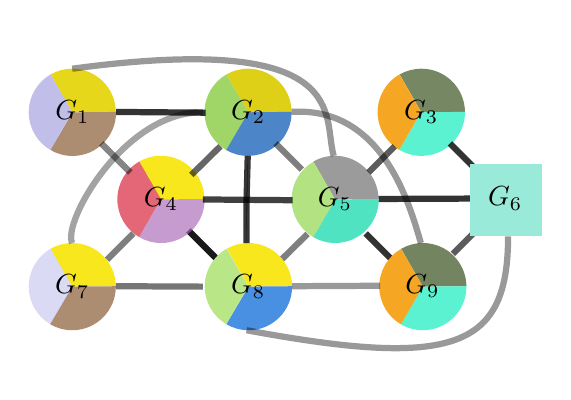
\begin{tikzpicture}[x=0.75pt,y=0.75pt,yscale=-0.7,xscale=0.7]
%uncomment if require: \path (0,1438); %set diagram left start at 0, and has height of 1438

%Straight Lines [id:da4186367162458817] 
\draw [color={rgb, 255:red, 0; green, 0; blue, 0 }  ,draw opacity=0.9 ][line width=2.25]    (248,1248) -- (270,1270) ;
%Straight Lines [id:da08988239364957362] 
\draw [color={rgb, 255:red, 0; green, 0; blue, 0 }  ,draw opacity=0.5 ][line width=2.25]    (310,1270) -- (330,1250.31) ;
%Straight Lines [id:da562224740054299] 
\draw [color={rgb, 255:red, 0; green, 0; blue, 0 }  ,draw opacity=0.8 ][line width=2.25]    (370,1250) -- (400,1280) ;
%Straight Lines [id:da5154222376250446] 
\draw [color={rgb, 255:red, 0; green, 0; blue, 0 }  ,draw opacity=0.8 ][line width=2.25]    (378.8,1226.26) -- (442,1226) ;
%Shape: Pie [id:dp22862520376005735] 
\draw  [draw opacity=0][fill={rgb, 255:red, 248; green, 231; blue, 28 }  ,fill opacity=1 ] (214.1,1200.48) .. controls (218.49,1197.96) and (223.58,1196.52) .. (229,1196.52) .. controls (245.48,1196.52) and (258.86,1209.81) .. (259,1226.26) -- (229,1226.52) -- cycle ;
%Shape: Pie [id:dp8772577465973821] 
\draw  [draw opacity=0][fill={rgb, 255:red, 170; green, 106; blue, 183 }  ,fill opacity=0.67 ] (259.19,1226.28) .. controls (259.19,1226.37) and (259.19,1226.47) .. (259.19,1226.57) .. controls (259.19,1243.14) and (245.76,1256.57) .. (229.19,1256.57) .. controls (223.62,1256.57) and (218.39,1255.05) .. (213.92,1252.4) -- (229.19,1226.57) -- cycle ;
%Shape: Pie [id:dp1897340912962322] 
\draw  [draw opacity=0][fill={rgb, 255:red, 208; green, 2; blue, 27 }  ,fill opacity=0.6 ] (213.92,1252.4) .. controls (205.03,1247.19) and (199.06,1237.54) .. (199.06,1226.49) .. controls (199.06,1215.37) and (205.11,1205.66) .. (214.1,1200.48) -- (229.06,1226.49) -- cycle ;
%Shape: Pie [id:dp5352410492568669] 
\draw  [draw opacity=0][fill={rgb, 255:red, 155; green, 155; blue, 155 }  ,fill opacity=1 ] (333.9,1200.48) .. controls (338.29,1197.96) and (343.38,1196.52) .. (348.81,1196.52) .. controls (365.29,1196.52) and (378.66,1209.81) .. (378.8,1226.26) -- (348.81,1226.52) -- cycle ;
%Shape: Pie [id:dp711098439811789] 
\draw  [draw opacity=0][fill={rgb, 255:red, 80; green, 227; blue, 194 }  ,fill opacity=1 ] (379,1226.28) .. controls (379,1226.37) and (379,1226.47) .. (379,1226.57) .. controls (379,1243.14) and (365.57,1256.57) .. (349,1256.57) .. controls (343.42,1256.57) and (338.2,1255.05) .. (333.73,1252.4) -- (349,1226.57) -- cycle ;
%Shape: Pie [id:dp7438737756485665] 
\draw  [draw opacity=0][fill={rgb, 255:red, 178; green, 226; blue, 130 }  ,fill opacity=1 ] (333.86,1252.48) .. controls (324.97,1247.27) and (319,1237.62) .. (319,1226.57) .. controls (319,1215.45) and (325.05,1205.74) .. (334.04,1200.56) -- (349,1226.57) -- cycle ;
%Shape: Pie [id:dp4950401144432839] 
\draw  [draw opacity=0][fill={rgb, 255:red, 34; green, 61; blue, 3 }  ,fill opacity=0.63 ] (394.43,1260.54) .. controls (398.82,1258.02) and (403.91,1256.58) .. (409.33,1256.58) .. controls (425.81,1256.58) and (439.18,1269.87) .. (439.33,1286.31) -- (409.33,1286.58) -- cycle ;
%Shape: Pie [id:dp32846163458006306] 
\draw  [draw opacity=0][fill={rgb, 255:red, 90; green, 242; blue, 208 }  ,fill opacity=1 ] (439.33,1286.31) .. controls (439.33,1286.41) and (439.33,1286.51) .. (439.33,1286.6) .. controls (439.33,1303.17) and (425.9,1316.6) .. (409.33,1316.6) .. controls (403.75,1316.6) and (398.53,1315.08) .. (394.06,1312.43) -- (409.33,1286.6) -- cycle ;
%Shape: Pie [id:dp6513356609327752] 
\draw  [draw opacity=0][fill={rgb, 255:red, 245; green, 166; blue, 35 }  ,fill opacity=1 ] (394.19,1312.51) .. controls (385.3,1307.3) and (379.33,1297.65) .. (379.33,1286.6) .. controls (379.33,1275.48) and (385.38,1265.78) .. (394.37,1260.6) -- (409.33,1286.6) -- cycle ;
%Shape: Pie [id:dp7206062426889672] 
\draw  [draw opacity=0][fill={rgb, 255:red, 248; green, 231; blue, 28 }  ,fill opacity=1 ] (274.43,1260.54) .. controls (278.82,1258.02) and (283.91,1256.58) .. (289.33,1256.58) .. controls (305.81,1256.58) and (319.18,1269.87) .. (319.33,1286.31) -- (289.33,1286.58) -- cycle ;
%Shape: Pie [id:dp8650493341112429] 
\draw  [draw opacity=0][fill={rgb, 255:red, 74; green, 144; blue, 226 }  ,fill opacity=1 ] (319.33,1286.31) .. controls (319.33,1286.41) and (319.33,1286.51) .. (319.33,1286.6) .. controls (319.33,1303.17) and (305.9,1316.6) .. (289.33,1316.6) .. controls (283.75,1316.6) and (278.53,1315.08) .. (274.06,1312.43) -- (289.33,1286.6) -- cycle ;
%Shape: Pie [id:dp3972433808884661] 
\draw  [draw opacity=0][fill={rgb, 255:red, 185; green, 231; blue, 136 }  ,fill opacity=1 ] (274.06,1312.43) .. controls (265.17,1307.22) and (259.19,1297.57) .. (259.19,1286.52) .. controls (259.19,1275.4) and (265.24,1265.7) .. (274.23,1260.52) -- (289.19,1286.52) -- cycle ;
%Shape: Pie [id:dp14987497027583996] 
\draw  [draw opacity=0][fill={rgb, 255:red, 34; green, 61; blue, 3 }  ,fill opacity=0.62 ] (393.43,1140.56) .. controls (397.82,1138.04) and (402.91,1136.6) .. (408.33,1136.6) .. controls (424.81,1136.6) and (438.19,1149.89) .. (438.33,1166.34) -- (408.33,1166.6) -- cycle ;
%Shape: Pie [id:dp6281781916199654] 
\draw  [draw opacity=0][fill={rgb, 255:red, 90; green, 242; blue, 208 }  ,fill opacity=1 ] (438.33,1166.31) .. controls (438.33,1166.41) and (438.33,1166.51) .. (438.33,1166.6) .. controls (438.33,1183.17) and (424.9,1196.6) .. (408.33,1196.6) .. controls (402.75,1196.6) and (397.53,1195.08) .. (393.06,1192.43) -- (408.33,1166.6) -- cycle ;
%Shape: Pie [id:dp7368216785514972] 
\draw  [draw opacity=0][fill={rgb, 255:red, 245; green, 166; blue, 35 }  ,fill opacity=1 ] (393.06,1192.43) .. controls (384.17,1187.22) and (378.19,1177.57) .. (378.19,1166.52) .. controls (378.19,1155.4) and (384.24,1145.7) .. (393.23,1140.52) -- (408.19,1166.52) -- cycle ;
%Shape: Pie [id:dp27649490289378686] 
\draw  [draw opacity=0][fill={rgb, 255:red, 222; green, 207; blue, 23 }  ,fill opacity=1 ] (274.1,1140.56) .. controls (278.49,1138.04) and (283.58,1136.6) .. (289,1136.6) .. controls (305.48,1136.6) and (318.86,1149.89) .. (319,1166.34) -- (289,1166.6) -- cycle ;
%Shape: Pie [id:dp8058575634583287] 
\draw  [draw opacity=0][fill={rgb, 255:red, 76; green, 133; blue, 200 }  ,fill opacity=1 ] (319,1166.31) .. controls (319,1166.41) and (319,1166.51) .. (319,1166.6) .. controls (319,1183.17) and (305.57,1196.6) .. (289,1196.6) .. controls (283.42,1196.6) and (278.2,1195.08) .. (273.73,1192.43) -- (289,1166.6) -- cycle ;
%Shape: Pie [id:dp5685252067895206] 
\draw  [draw opacity=0][fill={rgb, 255:red, 159; green, 214; blue, 103 }  ,fill opacity=1 ] (273.92,1192.48) .. controls (265.03,1187.27) and (259.06,1177.62) .. (259.06,1166.57) .. controls (259.06,1155.45) and (265.11,1145.74) .. (274.1,1140.56) -- (289.06,1166.57) -- cycle ;
%Shape: Pie [id:dp34533858656916694] 
\draw  [draw opacity=0][fill={rgb, 255:red, 231; green, 215; blue, 27 }  ,fill opacity=1 ] (153.1,1140.56) .. controls (157.49,1138.04) and (162.58,1136.6) .. (168,1136.6) .. controls (184.48,1136.6) and (197.86,1149.89) .. (198,1166.34) -- (168,1166.6) -- cycle ;
%Shape: Pie [id:dp6381985445084128] 
\draw  [draw opacity=0][fill={rgb, 255:red, 173; green, 141; blue, 113 }  ,fill opacity=1 ] (198.19,1166.36) .. controls (198.19,1166.45) and (198.19,1166.55) .. (198.19,1166.65) .. controls (198.19,1183.22) and (184.76,1196.65) .. (168.19,1196.65) .. controls (162.62,1196.65) and (157.39,1195.13) .. (152.92,1192.48) -- (168.19,1166.65) -- cycle ;
%Shape: Pie [id:dp9772609477611058] 
\draw  [draw opacity=0][fill={rgb, 255:red, 193; green, 191; blue, 234 }  ,fill opacity=1 ][line width=0.75]  (152.92,1192.48) .. controls (144.03,1187.27) and (138.06,1177.62) .. (138.06,1166.57) .. controls (138.06,1155.45) and (144.11,1145.74) .. (153.1,1140.56) -- (168.06,1166.57) -- cycle ;
%Shape: Pie [id:dp29151881669152435] 
\draw  [draw opacity=0][fill={rgb, 255:red, 248; green, 231; blue, 28 }  ,fill opacity=1 ] (153.1,1260.56) .. controls (157.49,1258.04) and (162.58,1256.6) .. (168,1256.6) .. controls (184.48,1256.6) and (197.86,1269.89) .. (198,1286.34) -- (168,1286.6) -- cycle ;
%Shape: Pie [id:dp5832605538270472] 
\draw  [draw opacity=0][fill={rgb, 255:red, 173; green, 141; blue, 113 }  ,fill opacity=1 ] (198,1286.31) .. controls (198,1286.41) and (198,1286.51) .. (198,1286.6) .. controls (198,1303.17) and (184.57,1316.6) .. (168,1316.6) .. controls (162.42,1316.6) and (157.2,1315.08) .. (152.73,1312.43) -- (168,1286.6) -- cycle ;
%Shape: Pie [id:dp04827723823086716] 
\draw  [draw opacity=0][fill={rgb, 255:red, 195; green, 193; blue, 236 }  ,fill opacity=0.6 ] (152.92,1312.48) .. controls (144.03,1307.27) and (138.06,1297.62) .. (138.06,1286.57) .. controls (138.06,1275.45) and (144.11,1265.74) .. (153.1,1260.56) -- (168.06,1286.57) -- cycle ;
%Straight Lines [id:da1744544159777348] 
\draw [color={rgb, 255:red, 0; green, 0; blue, 0 }  ,draw opacity=0.5 ][line width=2.25]    (192,1268) -- (210,1250) ;
%Straight Lines [id:da03935827821553706] 
\draw [color={rgb, 255:red, 0; green, 0; blue, 0 }  ,draw opacity=0.6 ][line width=2.25]    (250,1209.69) -- (270,1190) ;
%Straight Lines [id:da3827572200791203] 
\draw [color={rgb, 255:red, 0; green, 0; blue, 0 }  ,draw opacity=0.5 ][line width=2.25]    (308,1188) -- (326,1206) ;
%Straight Lines [id:da43054867062761004] 
\draw [color={rgb, 255:red, 0; green, 0; blue, 0 }  ,draw opacity=0.8 ][line width=2.25]    (428,1188) -- (450,1210) ;
%Straight Lines [id:da8030640791722374] 
\draw [color={rgb, 255:red, 0; green, 0; blue, 0 }  ,draw opacity=0.8 ][line width=2.25]    (198.19,1166.36) -- (259.89,1166.87) ;
%Straight Lines [id:da6075034403054509] 
\draw [color={rgb, 255:red, 0; green, 0; blue, 0 }  ,draw opacity=0.54 ][line width=2.25]    (198,1286.31) -- (258,1286.6) ;
%Straight Lines [id:da5065133384090603] 
\draw [color={rgb, 255:red, 0; green, 0; blue, 0 }  ,draw opacity=0.4 ][line width=2.25]    (319.33,1286.31) -- (380,1286) ;
%Straight Lines [id:da44694893447138084] 
\draw [color={rgb, 255:red, 0; green, 0; blue, 0 }  ,draw opacity=0.75 ][line width=2.25]    (258,1226.6) -- (319.7,1227.12) ;
%Straight Lines [id:da5494018194222325] 
\draw [color={rgb, 255:red, 0; green, 0; blue, 0 }  ,draw opacity=0.64 ][line width=2.25]    (372,1208) -- (390,1190) ;
%Straight Lines [id:da648544591287403] 
\draw [color={rgb, 255:red, 0; green, 0; blue, 0 }  ,draw opacity=0.64 ][line width=2.25]    (430,1264) -- (444,1250) ;
%Straight Lines [id:da8547781633391538] 
\draw [color={rgb, 255:red, 0; green, 0; blue, 0 }  ,draw opacity=0.79 ][fill={rgb, 255:red, 0; green, 0; blue, 0 }  ,fill opacity=1 ][line width=2.25]    (288,1256.6) -- (288,1226.6) -- (288.81,1196.57) ;
%Straight Lines [id:da010535895082270041] 
\draw [color={rgb, 255:red, 0; green, 0; blue, 0 }  ,draw opacity=0.48 ][line width=2.25]    (188,1188) -- (208,1208) ;
%Curve Lines [id:da9074501023534174] 
\draw [color={rgb, 255:red, 0; green, 0; blue, 0 }  ,draw opacity=0.4 ][line width=2.25]    (288,1316.6) .. controls (431.2,1343.2) and (467.95,1329.1) .. (468,1252) ;
%Curve Lines [id:da14318058563334723] 
\draw [color={rgb, 255:red, 0; green, 0; blue, 0 }  ,draw opacity=0.36 ][line width=2.25]    (168,1256.6) .. controls (160.84,1242.52) and (204.04,1165.72) .. (258,1166.6) ;
%Curve Lines [id:da07101319672858764] 
\draw [color={rgb, 255:red, 0; green, 0; blue, 0 }  ,draw opacity=0.4 ][line width=2.25]    (168,1136.6) .. controls (362.44,1110.52) and (340.04,1169.72) .. (348,1196.6) ;
%Curve Lines [id:da12269856496214393] 
\draw [color={rgb, 255:red, 0; green, 0; blue, 0 }  ,draw opacity=0.4 ][line width=2.25]    (319,1166.31) .. controls (381.64,1162.52) and (400.04,1229.72) .. (408,1256.6) ;
%Shape: Square [id:dp45069993806920583] 
\draw  [draw opacity=0][fill={rgb, 255:red, 153; green, 234; blue, 216 }  ,fill opacity=1 ] (442,1202) -- (491.5,1202) -- (491.5,1251.5) -- (442,1251.5) -- cycle ;

% Text Node
\draw (408.19,1166.52) node   [align=left] {$\displaystyle G_{3}$};
% Text Node
\draw (168,1286.6) node   [align=left] {$\displaystyle G_{7}$};
% Text Node
\draw (348.81,1226.52) node   [align=left] {$\displaystyle G_{5}$};
% Text Node
\draw (289.19,1286.52) node   [align=left] {$\displaystyle G_{8}$};
% Text Node
\draw (466,1226) node   [align=left] {$\displaystyle G_{6}$};
% Text Node
\draw (229,1226.52) node   [align=left] {$\displaystyle G_{4}$};
% Text Node
\draw (289.06,1166.54) node   [align=left] {$\displaystyle G_{2}$};
% Text Node
\draw (168.19,1166.65) node  [font=\normalsize] [align=left] {$\displaystyle G_{1}$};
% Text Node
\draw (409,1286.48) node   [align=left] {$\displaystyle G_{9}$};


\end{tikzpicture}
